\subsection{Data Processing and Preparation}

This subsection outlines our systematic approach to collecting, cleansing, and structuring data on fungal species and observations. In the following subsubsections you may find a detailed explanation of each of these tasks, as well as a conceptual data model and a reproducible pipeline.

\subsubsection{\textbf{Data Collection}}

As previously mentioned, structured data was sourced from GBIF, a reputable international data infrastructure. Two primary datasets were acquired: \texttt{occurrences}, which contains information regarding fungal species occurrences, and \texttt{multimedia}, which provides visual representations such as images and pictures associated with these occurrences. Both datasets were available in tab-separated values format. The \texttt{occurrences} dataset comprised over 700,000 rows and had a file size of 784 MB, whilst the \texttt{multimedia} dataset contained over 120,000 rows and had a file size of 28 MB. The data obtained from GBIF belong to different datasets, each with one of three licenses: \texttt{CC0 1.0}, \texttt{CC BY-NC 4.0} and \texttt{CC BY 4.0}, all of which permit the copy and redistribute the material in any medium or format and the remix, transform, and for us to build upon the material, as long as it's for non commercial purposes as per the \texttt{CC BY-NC 4.0} license. A list of all sampled datasets is provided in the annex.

In addition to structured data, our research encompasses the retrieval of unstructured data to enrich our information repository. This data includes the collection of abstracts from scientifically relevant articles on fungal species, as well as summarized content from Wikipedia pages dedicated to individual fungal species. The extraction of this data makes use of PubMed's (the database used for the querying of scientific articles) and Wikipedia's API's. For each species, a dedicated \texttt{JSON} file is created, which aggregates the contents of abstracts with the summary of their respective Wikipedia page.

\subsubsection{\textbf{Data Processing}}

From the \texttt{occurrences} dataset, we extracted a comprehensive list of all observed species. This list formed the foundation for a new dataset, specifically designed to capture essential species-related data, including taxonomic information such as kingdom, family, and vernacular (common) names. A second dataset dedicated to the records of species observations was generated from the trimmed \texttt{occurrences} dataset. To ensure data completeness and reduce redundancy, we merged features with identical semantic content. Key attributes, such as latitude, longitude, species name, and observation date, were integrated into this dataset. Finally, a third dataset was created to store visual representations associated with observations. This visual content was extracted from the \texttt{multimedia} dataset.

Following the creation of these datasets, they were subsequently loaded into a relational database. This database structure provides an efficient and structured platform for managing and querying the data.

\subsubsection{\textbf{Conceptual Data Model}}

The conceptual data model represents the main entities of our system: \texttt{SPECIES} (which contains species-specific information), \texttt{OBSERVATION} (which contains data about observations), \texttt{IMAGE} (which contains data about the visual representations of each image). The model is designed to provide a structured representation of the information, and \texttt{ABSTRACT} (which contains the contents of abstracts).

\begin{figure}[h]
  \centering
  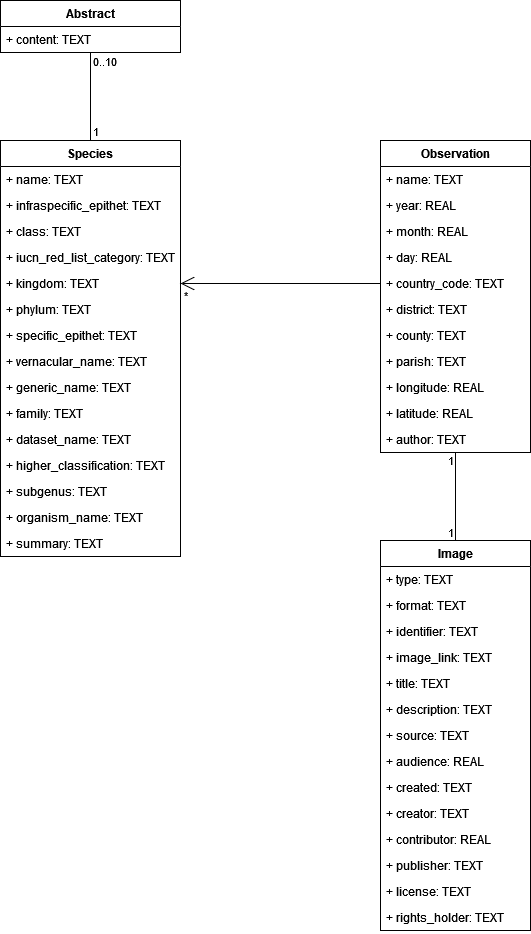
\includegraphics[width=0.5\linewidth]{figures/conceptual_data_model.drawio.png}
  \caption{Conceptual Data Model.}
  \Description{A Conceptual Data Model designed in UML, representing the main entities of the system.}
\end{figure}

\texttt{SPECIES} entity:
\begin{itemize}
    \item \texttt{name}: The name of the fungal species.
    \item \texttt{infraspecific\_epithet}: Additional taxonomic information specifying subspecies or variety.
    \item \texttt{class}: The taxonomic class of the species.
    \item \texttt{iucnRedList\_category}: The IUCN Red List category indicating the species' conservation status.
    \item \texttt{kingdom}: The taxonomic kingdom to which the species belongs.
    \item \texttt{phylum}: The taxonomic phylum of the species.
    \item \texttt{specific\_epithet}: Taxonomic information specifying the species within a genus.
    \item \texttt{vernacular\_name}: Common or colloquial name of the species.
    \item \texttt{generic\_name}: The generic or genus name to which the species belongs.
    \item \texttt{family}: The taxonomic family of the species.
    \item \texttt{dataset\_name}: Name of the dataset from which the species data originates.
    \item \texttt{higher\_classification}: Further taxonomic classification above the species level.
    \item \texttt{subgenus}: Taxonomic subgenus or subdivision.
    \item \texttt{organism\_name}: The name of the organism or species.
    \item \texttt{summary}: The summary of the Wikipedia page associated with the species.
\end{itemize}

\texttt{OBSERVATIONS} entity:
\begin{itemize}
    \item \texttt{name}: The name of the observed fungal species.
    \item \texttt{year}: The year of the observation.
    \item \texttt{month}: The month of the observation.
    \item \texttt{day}: The day of the observation.
    \item \texttt{country\_code}: The country code indicating the country of observation.
    \item \texttt{district}: The district where the observation took place.
    \item \texttt{county}: The county or regional division.
    \item \texttt{parish}: The specific parish or locality.
    \item \texttt{longitude}: The geographical longitude coordinates of the observation.
    \item \texttt{latitude}: The geographical latitude coordinates of the observation.
    \item \texttt{author}: The author or observer responsible for the observation.
\end{itemize}

\texttt{IMAGES} entity:
\begin{itemize}
    \item \texttt{type}: The type or category of the image.
    \item \texttt{format}: The file format or image format.
    \item \texttt{identifier}: An identifier for the image.
    \item \texttt{image\_link}: The link or reference to the image file.
    \item \texttt{title}: The title or caption associated with the image.
    \item \texttt{description}: A description or additional information about the image.
    \item \texttt{source}: The source or origin of the image.
    \item \texttt{audience}: The intended audience for the image.
    \item \texttt{created}: The date of creation or capture of the image.
    \item \texttt{creator}: The creator or author of the image.
    \item \texttt{contributor}: Contributions or additional contributors to the image.
    \item \texttt{publisher}: The publisher or source responsible for publishing the image.
    \item \texttt{license}: The license or usage terms associated with the image.
    \item \texttt{rights\_holder}: The rights holder or entity with rights to the image.
\end{itemize}

\texttt{ABSTRACT} entity:
\begin{itemize}
    \item \texttt{content}: The content of the abstract.
\end{itemize}

\subsubsection{\textbf{Data Pipeline}}

The data pipeline serves as the structured framework for our data preparation operations. It encompasses a sequence of designed steps to transform and refine raw data pertaining to fungal species, observations and content. Each stage within the pipeline fulfills a specific role, such as data extraction and cleansing. Conceptually, it operates as a structured workflow that systematically enhances the data's usability and accessibility. The figure below visually demonstrates the pipeline:

\begin{figure}[h]
  \centering
  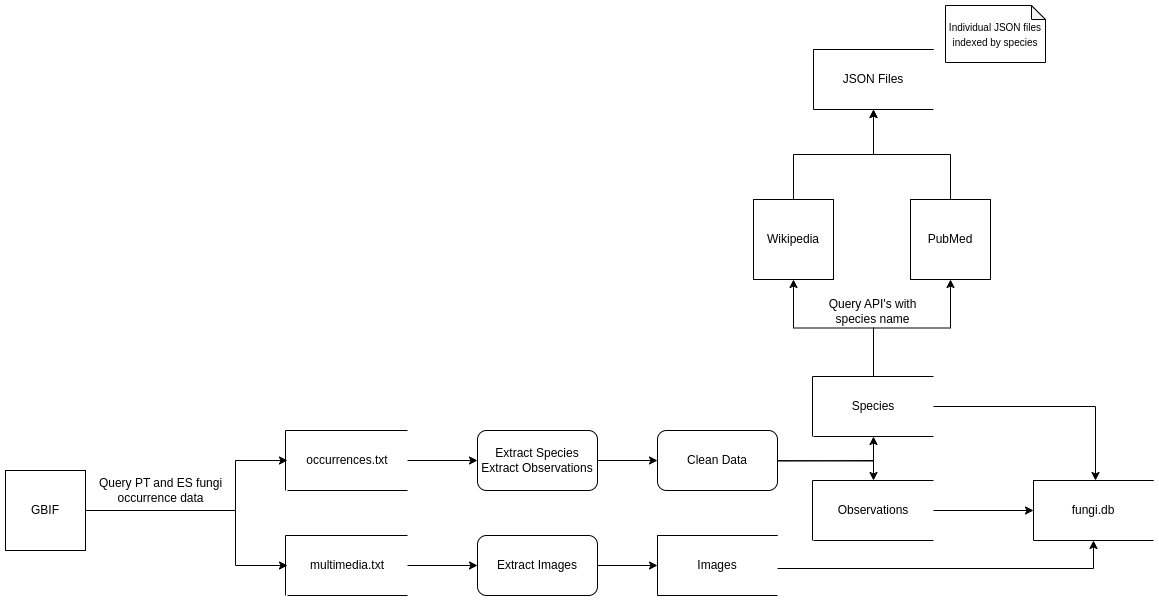
\includegraphics[width=\linewidth]{figures/data-flow-diagram.png}
  \caption{Data Pipeline.}
  \Description{The Data Pipeline, which demonstrates the order of operations on data.}
\end{figure}

To ensure that the entire data preparation process can be reliably recreated, the pipeline must be reproducible. In order to automate this process, a Makefile was designed. The Makefile enables us to automate and streamline the data preparation procedures from start to finish. 